% Exam Template for UMTYMP and Math Department courses
%
% Using Philip Hirschhorn's exam.cls: http://www-math.mit.edu/~psh/#ExamCls
%
% run pdflatex on a finished exam at least three times to do the grading table on front page.
%
%%%%%%%%%%%%%%%%%%%%%%%%%%%%%%%%%%%%%%%%%%%%%%%%%%%%%%%%%%%%%%%%%%%%%%%%%%%%%%%%%%%%%%%%%%%%%%

% These lines can probably stay unchanged, although you can remove the last
% two packages if you're not making pictures with tikz.
\documentclass[11pt]{exam}
\RequirePackage{amssymb, amsfonts, amsmath, latexsym, verbatim, xspace, setspace}
\RequirePackage{tikz, pgflibraryplotmarks}

% By default LaTeX uses large margins.  This doesn't work well on exams; problems
% end up in the "middle" of the page, reducing the amount of space for students
% to work on them.
\usepackage[margin=1in]{geometry}
\usepackage{enumerate}
\usepackage{amsthm}

\theoremstyle{definition}
\newtheorem{soln}{Solution}

% Here's where you edit the Class, Exam, Date, etc.
\newcommand{\class}{Math 150A Section 8 and 16}
\newcommand{\term}{Fall 2025}
\newcommand{\examnum}{Final Exam}
\newcommand{\examdate}{May 13, 2025}
\newcommand{\timelimit}{1 hour and 50 Minutes}

% For an exam, single spacing is most appropriate
\singlespacing
% \onehalfspacing
% \doublespacing

% For an exam, we generally want to turn off paragraph indentation
\parindent 0ex

\begin{document} 

% These commands set up the running header on the top of the exam pages
\pagestyle{head}
\firstpageheader{}{}{}
\runningheader{\class}{\examnum\ - Page \thepage\ of \numpages}{\examdate}
\runningheadrule

\begin{flushright}
\begin{tabular}{p{2.8in} r l}
\textbf{\class} & \textbf{Name (Print):} & \makebox[2in]{\hrulefill}\\
\textbf{\term} &&\\
\textbf{\examnum} & \textbf{Student ID:}&\makebox[2in]{\hrulefill}\\
\textbf{\examdate} &&\\
\textbf{Time Limit: \timelimit} % & Teaching Assistant & \makebox[2in]{\hrulefill}
\end{tabular}\\
\end{flushright}
\rule[1ex]{\textwidth}{.1pt}


This exam contains \numpages\ pages (including this cover page) and
\numquestions\ problems.  Check to see if any pages are missing.  Enter
all requested information on the top of this page, and put your initials
on the top of every page, in case the pages become separated.\\

You may \textit{not} use your books or notes on this exam.  However, you may use a single, handwritten, one-sided notesheet and a \textit{basic} calculator.\\

You are required to show your work on each problem on this exam, unless otherwise stated.
The following rules apply:\\

\begin{minipage}[t]{3.7in}
\vspace{0pt}
\begin{itemize}

%\item \textbf{If you use a ``fundamental theorem'' you must indicate this} and explain
%why the theorem may be applied.

\item \textbf{Organize your work}, in a reasonably neat and coherent way, in
the space provided. Work scattered all over the page without a clear ordering will 
receive very little credit.  

\item \textbf{Mysterious or unsupported answers will not receive full
credit}.  A correct answer, unsupported by calculations, explanation,
or algebraic work will receive no credit; an incorrect answer supported
by substantially correct calculations and explanations might still receive
partial credit.  This especially applies to limit calculations.

\item If you need more space, use the back of the pages; clearly indicate when you have done this.

\item \textbf{Box Your Answer} where appropriate, in order to clearly indicate what you consider the answer to the question to be.

\item Unless otherwise stated, all angles are in \textbf{radians}
\end{itemize}

Do not write in the table to the right.
\end{minipage}
\hfill
\begin{minipage}[t]{2.3in}
\vspace{0pt}
%\cellwidth{3em}
\gradetablestretch{2}
\vqword{Problem}
\addpoints % required here by exam.cls, even though questions haven't started yet.	
\gradetable[v]%[pages]  % Use [pages] to have grading table by page instead of question

\end{minipage}
\newpage % End of cover page

%%%%%%%%%%%%%%%%%%%%%%%%%%%%%%%%%%%%%%%%%%%%%%%%%%%%%%%%%%%%%%%%%%%%%%%%%%%%%%%%%%%%%
%
% See http://www-math.mit.edu/~psh/#ExamCls for full documentation, but the questions
% below give an idea of how to write questions [with parts] and have the points
% tracked automatically on the cover page.
%
%
%%%%%%%%%%%%%%%%%%%%%%%%%%%%%%%%%%%%%%%%%%%%%%%%%%%%%%%%%%%%%%%%%%%%%%%%%%%%%%%%%%%%%

\begin{questions}

\addpoints

\question[20]\mbox{}
\textbf{TRUE or FALSE!}
If the statement is true, write TRUE (all caps, all spelled out).
Otherwise write FALSE (all caps, all spelled out).
\begin{enumerate}[(a)]
\item the function $f(x) = e^x$ has a critical point
\vspace{0.6in}
\item $x^2$ has an inflection point at $x=0$
\vspace{0.6in}
\item if $f(x)$ is continuous at $x=2$, then it is differentiable at $x=2$
\vspace{0.6in}
\item if $f'(1) = 2$ and $g'(1) = 3$, then the derivative of $f(g(x))$ at $x=1$ is $6$
\vspace{0.6in}
\item $\tan(\tan^{-1}(10)) = 10$
\vspace{0.6in}
\item $\int_0^1 2f(x)dx = 2\int_0^1 f(x) dx$
\vspace{0.6in}
\item $\frac{d}{dx}e^{2x} = 2e^{2x}$
\vspace{0.6in}
\item if $f(x)$ is differentiable and $f'(x) = 0$, then $f(x)$ is a constant
\vspace{0.6in}
\item the function $e^x+x$ has a root in the interval $[0,2]$
\vspace{0.6in}
\item a function can only have one vertical asymptote
\end{enumerate}

\newpage
\question[10]\mbox{}
Calculate the following.  Carefully show you work.
\begin{enumerate}[(a)]
\item $\lim_{x\rightarrow 2}\frac{x^2-5x+6}{x^2-4}$
\vspace{2in}
\item $\lim_{x\rightarrow \infty}\sqrt{x^2+1}-\sqrt{x^2+2x}$
\vspace{2in}
\item $\lim_{x\rightarrow 0} \frac{e^{2x}-1}{3x}$
\vspace{2in}
\item $\lim_{x\rightarrow \infty} (1+5x)^{1/x}$
\vspace{2in}
\end{enumerate}

\newpage
\question[10]
The following is a graph of the \textbf{derivative} $f'(x)$ of a function $f(x)$.
\begin{center}
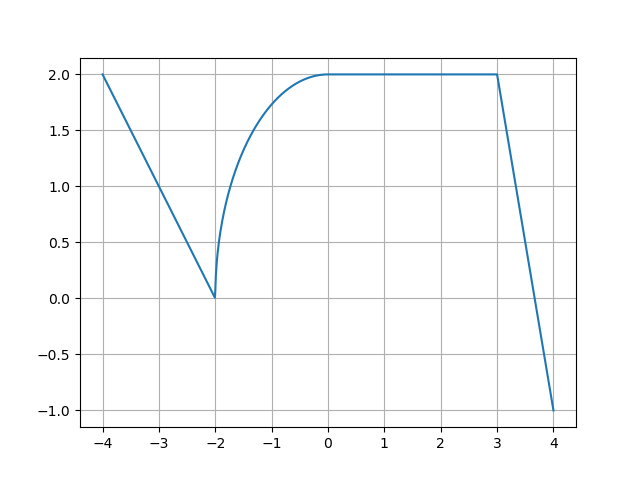
\includegraphics[width=.7\linewidth]{fig/finalfig.png}
\end{center}
\begin{enumerate}[(a)]
\item List all intervals where $f(x)$ is concave down
\vspace{1in}
\item List all critical points of $f(x)$ and classify them as local max, local min or neither
\vspace{1in}
\item What is $\lim_{x\rightarrow -3} \frac{f'(x)}{x+3}$?
\vspace{1in}
\item If $f(-4) = 1$, what is the value of $f(3)$?  Assume $f(x) = \sqrt{4-x^2}$ for $-2\leq x \leq 0$
\end{enumerate}

\newpage
\question[10]\mbox{}
\begin{enumerate}
\item  Find all critical points of the function $f(x) = \frac{e^x-1}{e^{2x}+1}$
\vspace{3.5in}
\item  If $f(2) = 0.75$ and $f'(2) = -0.25$, use the linearization of $f(x)$ at $x=2$ to estimate $f(1.9)$.
\end{enumerate}


\newpage
\question[10]\mbox{}
Find the derivative of each of the following functions.
\begin{enumerate}[(a)]
\item  $x\tan^{-1}(x^2)$
\vspace{2.5in}
\item  $\frac{\cos(x)}{x+2^x}$
\vspace{2.5in}
\item  $x^x$
\end{enumerate}

\newpage
\question[10]
Consider a rectangular box with a square base, an open top, and a volume of $216$ cubic inches. 
What dimensions minimize the surface area of the box?  What is the minimum surface area?

\newpage
\question[10]
Find the area of the region bounded by $y = -x^2+10$ and $y= (x-2)^2$.

\newpage
\question[10]
Compute each of the following integrals.  Show all work.
Lack of work results in no credit!!
\begin{enumerate}[(a)]
\item $\int_1^8 \frac{3 + t}{t}dt$
\vspace{2in}
\item $\int 2xe^{x^2}dx$
\vspace{2in}
\item $\int  \frac{e^s}{1 + e^{2s}}ds$
\vspace{2in}
\item $\int_0^3 (x^3 + 3^x) dx$
\end{enumerate}




\end{questions}
\end{document}

